\textbf{5-1.} 电动势为 $12\mathrm{V}$ 的汽车电池的内阻为 $0.05\Omega$ ，问：

(1) 它的短路电流多大?

(2) 若启动电流为 100A, 则启动马达的内阻多大?

\vfill
\textbf{5-2.} 如本题图所示，在电动势为 $\mathcal{E}$ 、内阻为 $r$ 的电池上连接一个 $R_{1} = 10.0\Omega$ 的电阻时，测出 $R_{1}$ 的端电压为 $8.0\mathrm{V}$ ，若将 $R_{1}$ 换成 $R_{2} = 5.0\Omega$ 的电阻时，其端电压为 $6.0\mathrm{V}$ . 求此电池的 $\mathcal{E}$ 和 $r$ .
\begin{center}
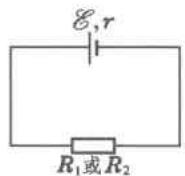
\includegraphics[width=0.25\linewidth]{figures/习题5-2.jpg}
\end{center}

\vfill
\newpage

\textbf{5-3.} 试推导当气体中有正负两种离子参与导电时，电流密度的公式为

$$
\boldsymbol {j} = n _ {+} q _ {+} \boldsymbol {u} _ {+} + n _ {-} q _ {-} \boldsymbol {u} _ {-},
$$

式中 $n_{+}, q_{+}, u_{+}$ 分别代表正离子的数密度、所带电量和漂移速度， $n_{-}, q_{-}$

$u_{-}$ 分别代表负离子的相应量。
\begin{center}
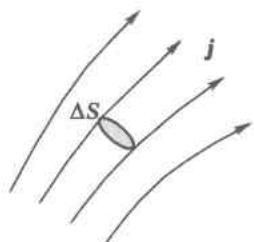
\includegraphics[width=0.25\linewidth]{figures/习题5-3.jpg}
\end{center}

\vfill
\textbf{5-4.} 在地面附近的大气里，由于土壤的放射性和宇宙线的作用，平均每 $1\mathrm{cm}^3$ 的大气里约有5对离子。离子的漂移速度正比于场强，比例系数称为“迁移率”。已知大气中正离子的迁移率为 $1.37\times 10^{-4}\mathrm{m}^2 /\left(\mathrm{s}\cdot \mathrm{V}\right)$ 负离子的迁移率为 $1.91\times 10^{-4}\mathrm{m}^2 /\left(\mathrm{s}\cdot \mathrm{V}\right)$ ，正负离子所带的电荷量数值都是 $1.60 \times 10^{-19}$ C. 求地面大气的电导率 $\sigma$ .

\vfill
\newpage

\textbf{5-5.} 空气中有一对平行放着的极板，相距 $2.00\mathrm{cm}$ ，面积都是 $300\mathrm{cm}^2$ 。在两板上加 $150\mathrm{V}$ 的电压，这个值远小于使电流达到饱和所需的电压。今用X射线照射板间的空气，使其电离，于是两板间便有 $4.00\mu \mathrm{A}$ 的电流通过。设正负离子的电量都是 $1.60\times 10^{-19}\mathrm{C}$ ，已知其中正离子的迁移率为 $1.37\times 10^{-4}\mathrm{m}^2 /(\mathrm{s}\cdot \mathrm{V})$ ，负离子的迁移率为 $1.91\times 10^{-4}\mathrm{m}^2 /(\mathrm{s}\cdot \mathrm{V})$ ，求这时板间离子的浓度。

\vfill
\textbf{5-6.} 四个电阻均为 $6.0\Omega$ 的灯泡，工作电压为 $12\mathrm{V}$ ，把它们并联起来接到一个电动势为 $12\mathrm{V}$ 、内阻为 $0.20\Omega$ 的电源上。问：

(1) 开一盏灯时, 此灯两端的电压多大?

(2) 四盏灯全开, 灯两端的电压多大?

\vfill
\newpage

\textbf{5-7.} 本题图中伏特计的内阻为 $300\Omega$ ，在开关K未合上时其电压读数为1.49V，开关合上时其读数为1.46V，求电源的电动势和内阻。
\begin{center}
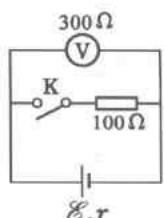
\includegraphics[width=0.25\linewidth]{figures/习题5-7.jpg}
\end{center}

\vfill
\textbf{5-8.} 变阻器可用作分压器，用法如本题图所示。 $U$ 是输入电压， $R$ 是变阻器的全电阻， $r$ 是负载电阻， $c$ 是 $R$ 上的滑动接头。滑动 $c$ ，就可以在负载上得到从0到 $U$ 之间的任何电压 $U_{r}$ 。设 $R$ 的长度 $ab = l$ ， $R$ 上各处单位长度的电阻都相同， $a, c$ 之间的长度 $ac = x$ ，求加到 $r$ 上的电压 $U_{r}$ 与 $x$ 的关系。用方格纸画出当 $r = 0.1R$ 和 $r = 10R$ 时的 $U_{r} - x$ 曲线。
\begin{center}
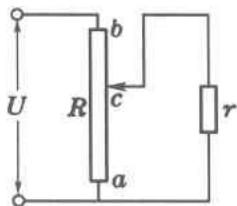
\includegraphics[width=0.25\linewidth]{figures/习题5-8a.jpg}
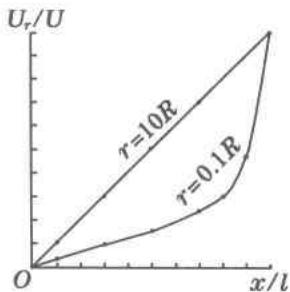
\includegraphics[width=0.25\linewidth]{figures/习题5-8b.jpg}
\end{center}

\vfill
\newpage

\textbf{5-9.} 在本题图所示的电路中, 求: (1) $R_{CD}$ , (2) $R_{BC}$ , (3) $R_{AB}$ .
\begin{center}
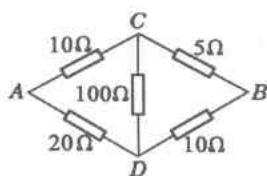
\includegraphics[width=0.4\linewidth]{figures/习题5-9.jpg}
\end{center}

\vfill
\textbf{5-10.} 判断一下，在本题图中所示各电路中哪些可以化为串、并联电路的组合，哪些不能。如果可以，就利用串、并联公式写出它们总的等效电阻。
\begin{center}
\begin{tabular}{cc}
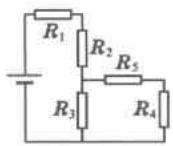
\includegraphics[width=0.2\linewidth]{figures/习题5-10a.jpg} & 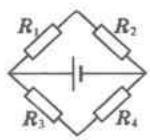
\includegraphics[width=0.2\linewidth]{figures/习题5-10b.jpg} \\
\end{tabular}
\begin{tabular}{cc}
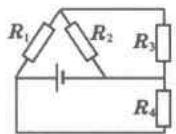
\includegraphics[width=0.2\linewidth]{figures/习题5-10c.jpg} & 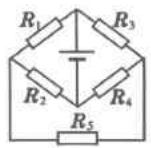
\includegraphics[width=0.2\linewidth]{figures/习题5-10d.jpg} \\
\end{tabular}
\begin{tabular}{cc}
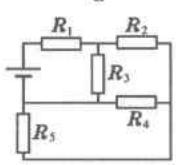
\includegraphics[width=0.2\linewidth]{figures/习题5-10e.jpg} & 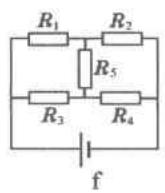
\includegraphics[width=0.2\linewidth]{figures/习题5-10f.jpg} \\
\end{tabular}
\begin{tabular}{cc}
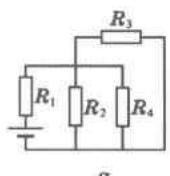
\includegraphics[width=0.2\linewidth]{figures/习题5-10g.jpg} & 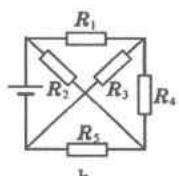
\includegraphics[width=0.2\linewidth]{figures/习题5-10h.jpg} \\
\end{tabular}
\end{center}

\vfill
\newpage

\textbf{5-11.} 无轨电车速度的调节, 是依靠在直流电动机的回路中串入不同数值的电阻, 以改变通过电动机的电流, 使电动机的转速发生变化。例如, 可以在回路中串接四个电阻 $R_{1}, R_{2}, R_{3}$ 和 $R_{4}$ , 再利用一些开关 $\mathrm{K}_{1}, \mathrm{K}_{2}, \mathrm{K}_{3}, \mathrm{K}_{4}$ 和 $\mathrm{K}_{5}$ , 使电阻分别串联或并联，以改变总电阻的数值，如本题图中所示。设 $R_{1}=R_{2}=R_{3}=R_{4}=1.0\Omega$ ，求下列四种情况下的等效电阻 $R_{ab}$ ：

(1) $K_{1}$ 、 $K_{5}$ 合上， $K_{2}$ 、 $K_{3}$ 、 $K_{4}$ 断开；

(2) $K_{2}$ 、 $K_{3}$ 、 $K_{5}$ 合上， $K_{1}$ 、 $K_{4}$ 断开；

(3) $K_{1}$ 、 $K_{3}$ 、 $K_{4}$ 合上， $K_{2}$ 、 $K_{5}$ 断开；

(4) $K_{1}$ 、 $K_{2}$ 、 $K_{3}$ 、 $K_{4}$ 合上， $K_{5}$ 断开。
\begin{center}
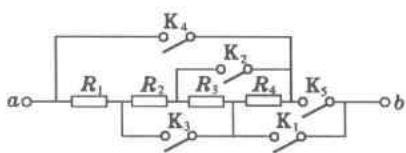
\includegraphics[width=0.4\linewidth]{figures/习题5-11.jpg}
\end{center}

\vfill
\textbf{5-12.} 本题图所示电路, U=12V, $R_{1}=30k\Omega$ , $R_{2}=6.0k\Omega$ , $R_{3}=100k\Omega$ , $R_{4}=10k\Omega$ , $R_{5}=100k\Omega$ , $R_{6}=1.0k\Omega$ , $R_{7}=2.0k\Omega$ , 求电压 $U_{ab}$ , $U_{ac}$ , $U_{ad}$ .
\begin{center}
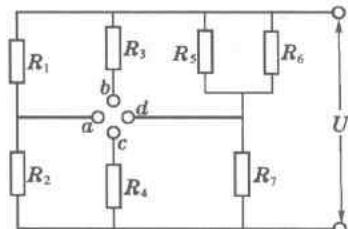
\includegraphics[width=0.3\linewidth]{figures/习题5-12.jpg}
\end{center}

\vfill
\newpage

\textbf{5-13.} MF-5型万用电表的电流挡为闭路抽头式的，如本题图所示。表头的内阻 $R_{\mathrm{G}} = 2333\Omega$ ，满度电流 $I_{\mathrm{G}} = 150\mu \mathrm{A}$ ，将其改装为量程是 $500\mu \mathrm{A}$ 、 $10\mathrm{mA}$ 、 $100\mathrm{mA}$ 试算出 $R_{1},R_{2},R_{3}$ 的阻值，并标出三个接头的量程。
\begin{center}
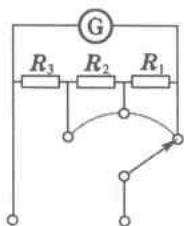
\includegraphics[width=0.25\linewidth]{figures/习题5-13.jpg}
\end{center}

\vfill
\textbf{5-14.} MF-5型万用电表的电压挡如本题图所示，表头满度电流 $I_{G}=0.50mA$ ，内阻 $R_{G}=700\Omega$ ，改装为多量程伏特计的量程分别为 $U_{1}=10V$ ， $U_{2}=50V$ ， $U_{3}=250V$ ，求各挡的降压电阻 $R_{1}$ 、 $R_{2}$ 、 $R_{3}$ 。若再增加两个量程 $U_{4}=500V$ ， $U_{5}=1000V$ ，又该如何？
\begin{center}
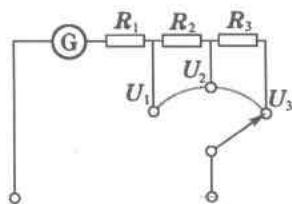
\includegraphics[width=0.25\linewidth]{figures/习题5-14.jpg}
\end{center}

\vfill
\newpage

\textbf{5-15.} 甲乙两站相距 $50\mathrm{km}$ , 其间有两条相同的电话线, 有一条因在某处触地而发生故障, 甲站的

检修人员用本题图所示的办法找出触地到甲站的距离 x，让乙站把两条电话线短路，调节 r 使通过检流计 G 的电流为 0。已知电话线每 km 长的电阻为 $6.0 \Omega$ ，测得 $r = 360 \Omega$ ，求 x。
\begin{center}
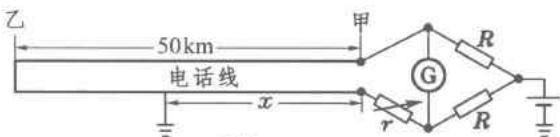
\includegraphics[width=0.4\linewidth]{figures/习题5-15.jpg}
\end{center}

\vfill
\textbf{5-16.} 为了找出电缆在某处由于损坏而通地的地方，也可以用本题图所示的装置。 $AB$ 是一条长为 $100\mathrm{cm}$ 的均匀电阻线，接触点 $S$ 可在它上面

滑动。已知电缆长7.8km，设当S滑到SB=41cm时，通过电流计G的电

流为0. 求电缆损坏处到B的距离x.
\begin{center}
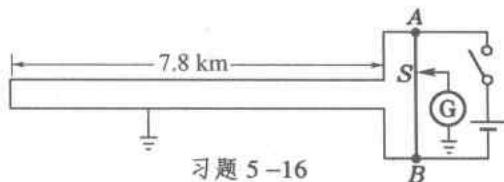
\includegraphics[width=0.4\linewidth]{figures/习题5-16.jpg}
\end{center}

\vfill
\newpage

\textbf{5-17.} 一电路如本题图，已知 $\mathcal{E}_1 = 1.5\mathrm{V}$ ， $\mathcal{E}_2 = 1.0\mathrm{V}$ ， $R_1 = 50\Omega$ ， $R_2 = 80\Omega$ ， $R = 10\Omega$ ，电池的内阻都可忽略不计。求通过 $R$ 的电流。
\begin{center}
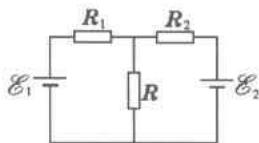
\includegraphics[width=0.4\linewidth]{figures/习题5-17.jpg}
\end{center}

\vfill
\textbf{5-18.} 一电路如本题图，已知 $\mathcal{E}_1 = 12\mathrm{V}$ ， $\mathcal{E}_2 = 9\mathrm{V}$ ， $\mathcal{E}_3 = 8\mathrm{V}$ ， $r_1 = r_2 = r_3 = 1\Omega$ ， $R_1 = R_3 = R_4 = R_5 = 2\Omega$ ， $R_2 = 3\Omega$ 。求：

(1) a、b 断开时的 $U_{ab}$ ;

(2) a、b 短路时通过 $E_{2}$ 的电流的大小和方向。
\begin{center}
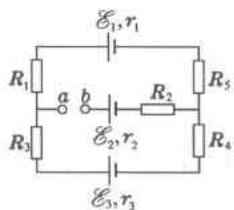
\includegraphics[width=0.3\linewidth]{figures/习题5-18a.jpg}
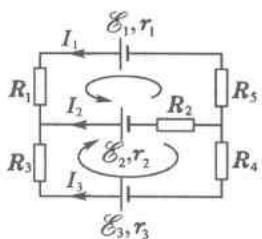
\includegraphics[width=0.3\linewidth]{figures/习题5-18b.jpg}
\end{center}

\vfill
\newpage

\textbf{5-19.} 一电路如本题图, 已知 $\mathcal{E}_1 = 1.0\mathrm{V}$ , $\mathcal{E}_2 = 2.0\mathrm{V}$ , $\mathcal{E}_3 = 3.0\mathrm{V}$ , $r_1 = r_2 = r_3 = 1.0\Omega$ , $R_1 = 1.0\Omega$ , $R_2 = 3.0\Omega$ . 求:

(1) 通过电源 3 的电流；

(2) $R_{2}$ 消耗的功率；

(3) 电源 3 对外供给的功率。

\begin{center}
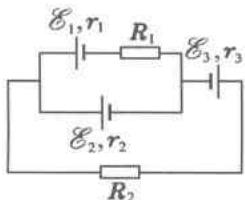
\includegraphics[width=0.3\linewidth]{figures/习题5-19a.jpg}
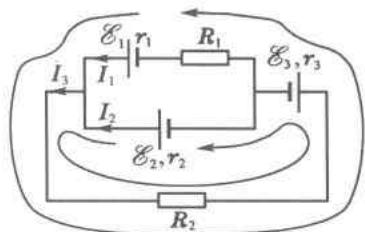
\includegraphics[width=0.3\linewidth]{figures/习题5-19b.jpg}
\end{center}

\vfill
\textbf{5-20.} 分别求出本题图 a、b、c 中 a、b 间的电阻。
\begin{center}
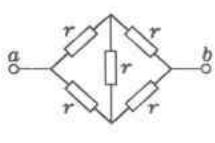
\includegraphics[width=0.25\linewidth]{figures/习题5-20a.jpg}
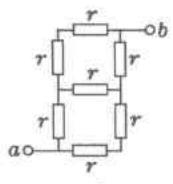
\includegraphics[width=0.25\linewidth]{figures/习题5-20b.jpg}
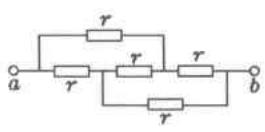
\includegraphics[width=0.25\linewidth]{figures/习题5-20c.jpg}
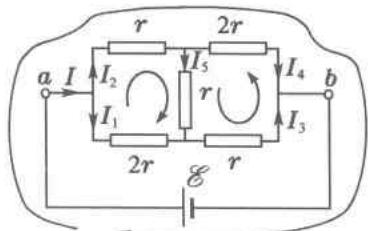
\includegraphics[width=0.25\linewidth]{figures/习题5-20d.jpg}
\end{center}

\vfill
\newpage

\textbf{5-21.} 将本题图中的电压源变换成等效的电流源。
\begin{center}
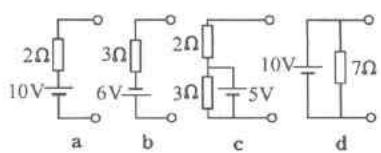
\includegraphics[width=0.4\linewidth]{figures/习题5-21.jpg}
\end{center}

\vfill
\textbf{5-22.} 将本题图中的电流源转换成等效的电压源。
\begin{center}
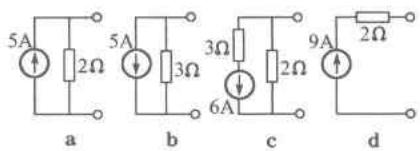
\includegraphics[width=0.4\linewidth]{figures/习题5-22.jpg}
\end{center}

\vfill
\newpage

\textbf{5-23.} 用等效电源定理解习题 5-18 中的(2)。
\begin{center}
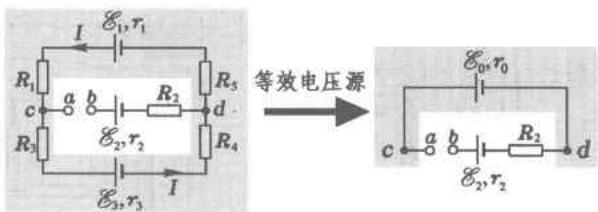
\includegraphics[width=0.45\linewidth]{figures/习题5-23.jpg}
\end{center}

\vfill
\textbf{5-24.} 用等效电源定理求图 5-32 中电桥电路的 $I_{\mathrm{G}}$

\vfill
\newpage

\textbf{5-25.} 求本题图中 $ab$ 支路中的电流。
\begin{center}
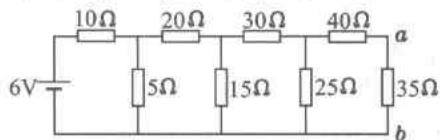
\includegraphics[width=0.4\linewidth]{figures/习题5-25.jpg}
\end{center}

\vfill
\textbf{5-26.} 证明 $L / R$ 和 $RC$ 具有时间的量纲，并且 $1\mathrm{H} / 1\Omega = 1\mathrm{s}$ ， $1\Omega \cdot 1\mathrm{F} = 1\mathrm{s}$ .



\vfill
\newpage

\textbf{5-27.} 一个自感为 $0.50 \mathrm{~mH}$ 、电阻为 $0.01 \Omega$ 的线圈连接到内阻可忽略、电动势为 $12 \mathrm{~V}$ 的电源上。开关接通多长时间，电流达到终值的 $90 \%$ ？到此时线圈中储存了多少能量？电源消耗了多少能量？

\vfill
\textbf{5-28.} 一自感为 $L$ 、电阻为 $R$ 的线圈与一无自感的电阻 $R_0$ 串联地接于电源上，如本题图所示。

(1) 求开关 $K_{1}$ 闭合 t 时间后，线圈两端的电势差 $U_{bc}$ ;

(2) 若 $\mathcal{E}=20\mathrm{V}, R_{0}=50\Omega, R=150\Omega, L=5.0\mathrm{H}$ ，求 $t=0.5\tau$ 时（ $\tau$ 为电路的时间常量）线圈两端的电势差 $U_{bc}$ 和 $U_{ab}$ ;

(3) 待电路中电流达到稳定值，闭合开关 $K_{2}$ ，求闭合 0.01 s 后通过 $K_{2}$ 中电流的大小和方向。

\begin{center}
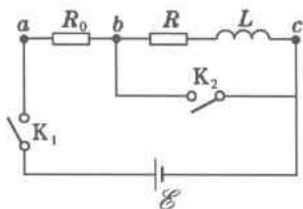
\includegraphics[width=0.3\linewidth]{figures/习题5-28.jpg}
\end{center}

\vfill
\newpage

\textbf{5-29.} 一电路如本题图所示， $R_{1}, R_{2}, L$ 和 $\mathcal{E}$ 都已知，电源 $\mathcal{E}$ 和线圈 $L$ 的内阻都可略去不计。

(1) 求 K 接通后，a、b 间的电压与时间的关系；

(2) 在电流达到最后稳定值的情况下, 求 K 断开后 a、b 间的电压与时间的关系。
\begin{center}
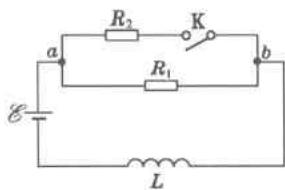
\includegraphics[width=0.25\linewidth]{figures/习题5-29.jpg}
\end{center}

\vfill
\textbf{5-30.} 两线圈之间的互感为 $M$ ，电阻分别为 $R_{1}$ 和 $R_{2}$ ，第一个线圈接在电动势为 $\mathcal{E}$ 的电源上，第二个线圈接在电阻为 $R_{\mathrm{G}}$ 的电流计 $\mathrm{G}$ 上，如本题图所示。设开关 $\mathbf{K}$ 原先是接通的，第二个线圈内无电流，然后把 $\mathbf{K}$ 断开。

(1) 求通过电流计 G 的电量 q;

(2) q 与两线圈的自感有什么关系?
\begin{center}
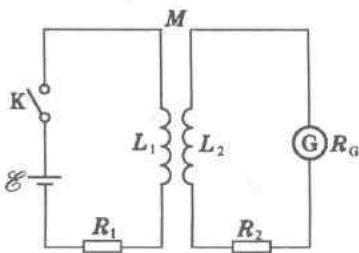
\includegraphics[width=0.25\linewidth]{figures/习题5-30.jpg}
\end{center}

\vfill
\newpage

\textbf{5-31.} 本题图示为一对互感耦合的 $LR$ 电路。证明在无漏磁的条件下两回路充放电的时间常量都是

$$
\tau = \frac {L _ {1}}{R _ {1}} + \frac {L _ {2}}{R _ {2}}.
$$

由此定性地解释,为什么当电感元件的铁芯中若有涡流时,电路充放电的时间常量要增大？

【提示:列出两回路的电路方程,这是一组联立的一阶线性微分方程组,解此方程组即可求得。】
\begin{center}
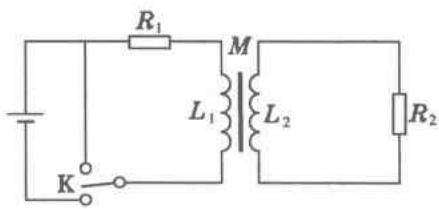
\includegraphics[width=0.4\linewidth]{figures/习题5-31.jpg}
\end{center}

\vfill
\textbf{5-32.} 在 $LC$ 振荡回路中，设开始时 $C$ 上的电荷量为 $Q, L$ 中的电流为0.

(1) 求第一次达到 L 中磁能等于 C 中电能所需的时间 t;

(2) 求这时 C 上的电荷量 q.

\vfill
\newpage

\textbf{5-33.} 两个 $C = 2.0\mu \mathrm{F}$ 的电容器已充有相同的电荷量，经过一线圈（ $L = 1.0\mathrm{mH}, R = 50\Omega$ ）放电。问当这两个电容器（1）并联时，（2）串联时，能不能发生振荡。

\vfill
\textbf{5-34.} 在同一时间坐标轴上画出简谐交流电压 $u_{1}(t) = 311\cos (314t - 2\pi /3)\mathrm{V}$ 和 $u_{2}(t) = 311\sin (314t - 5\pi /6)\mathrm{V}$ 的曲线。它们的峰值、有效值、频率和相位各多少？哪个超前？
\begin{center}
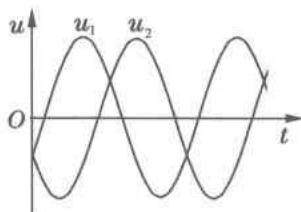
\includegraphics[width=0.4\linewidth]{figures/习题5-34.jpg}
\end{center}

\vfill
\newpage

\textbf{5-35.} 两个简谐交流电 $i_1(t)$ 和 $i_2(t)$ 的波形如本题图所示，

(1) 写出它们的三角函数(余弦)表达式,

（2）它们之间的相位差为多少？哪个超前？
\begin{center}
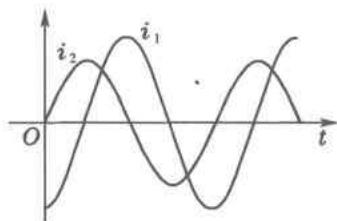
\includegraphics[width=0.4\linewidth]{figures/习题5-35.jpg}
\end{center}

\vfill
\textbf{5-36.} 电阻 $R$ 的单位为 $\Omega$ , 自感 $L$ 的单位为 $\mathrm{H}$ , 电容 $C$ 的单位为 $\mathbf{F}$ , 频率 $\nu$ 的单位为 $\mathrm{Hz}$ , 角频率 $\omega = 2\pi \nu$ . 证明 $\omega L, 1 / \omega C$ 的单位为 $\Omega$ .

\vfill
\newpage

\textbf{5-37.} (1) 分别求频率为 50 Hz 和 500 Hz 时 10 H 电感的阻抗。

(2) 分别求频率为 $50 \, Hz$ 和 $500 \, Hz$ 时 $10 \, \mu F$ 电容的阻抗。

(3) 在哪一个频率时, $10 \mathrm{H}$ 电感器的阻抗等于 $10 \mu \mathrm{F}$ 电容器的阻抗?

\vfill
\textbf{5-38.} 已知在某频率下本题图中电容、电阻的阻抗数值之比为

$$
Z _ {C}: Z _ {R} = 3: 4,
$$

若在串联电路两端加总电压 U = 100 V,

(1) 电容和电阻元件上的电压 $U_{C}$ 、 $U_{R}$ 为多少？

(2) 电阻元件中的电流与总电压之间有无相位差?
\begin{center}
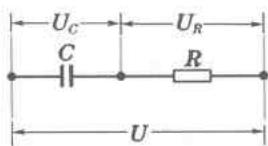
\includegraphics[width=0.35\linewidth]{figures/习题5-38a.jpg}
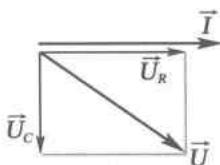
\includegraphics[width=0.35\linewidth]{figures/习题5-38b.jpg}
\end{center}

\vfill
\newpage

\textbf{5-39.} 已知在某频率下本题图中电感和电容元件阻抗数值之比为

$$
Z _ {L}: Z _ {C} = 2: 1,
$$

总电流 I=1mA，问通过 L 和 C 的电流 $I_{L}$ 、 $I_{C}$ 各多少？
\begin{center}
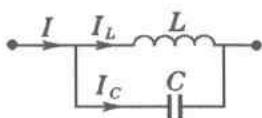
\includegraphics[width=0.4\linewidth]{figures/习题5-39.jpg}
\end{center}

\vfill
\textbf{5-40.} 在本题图中 $U_{1} = U_{2} = 20\mathrm{V}, Z_{C} = R_{2}$ ，求总电压 U.
\begin{center}
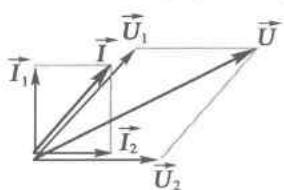
\includegraphics[width=0.3\linewidth]{figures/习题5-40a.jpg}
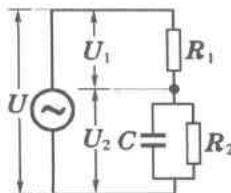
\includegraphics[width=0.3\linewidth]{figures/习题5-40b.jpg}
\end{center}

\vfill
\newpage

\textbf{5-41.} 在上题图中已知 $U_{1} = U_{2}$ , $Z_{C}:R_{2} = 1:\sqrt{3}$ , 用矢量图解法求总电压与总电流的相位差。
\begin{center}
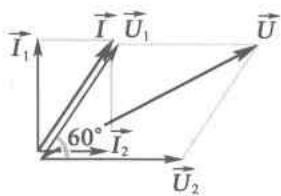
\includegraphics[width=0.3\linewidth]{figures/习题5-41.jpg}
\end{center}

\vfill
\textbf{5-42.} 在本题图中已知 $Z_{L}: Z_{C}: R = 2:1:1$ ，求：

(1) $I_{1}$ 与 $I_{2}$ 间的相位差，

(2) U 与 $U_{c}$ 间的相位差，并用矢量图说明之。
\begin{center}
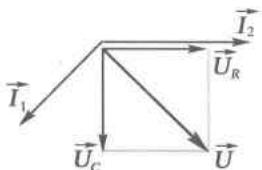
\includegraphics[width=0.3\linewidth]{figures/习题5-42a.jpg}
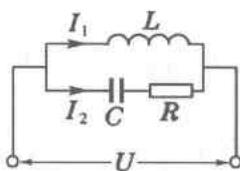
\includegraphics[width=0.3\linewidth]{figures/习题5-42b.jpg}
\end{center}

\vfill
\newpage

\textbf{5-43.} 在本题图中 $Z_{L} = Z_{C} = R$ ，求下列各量间的相位差，并用矢量图说明之：

(1) $U_{C}$ 与 $U_{R}$ ;

(2) $I_{C}$ 与 $I_{R}$ ;

(3) $U_{R}$ 与 $U_{L}$ ;

(4) $U$ 与 $I$ .
\begin{center}
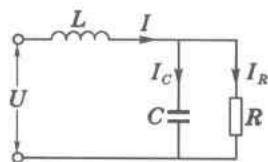
\includegraphics[width=0.3\linewidth]{figures/习题5-43a.jpg}
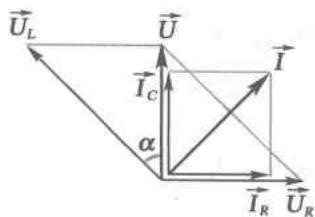
\includegraphics[width=0.3\linewidth]{figures/习题5-43b.jpg}
\end{center}

\vfill
\textbf{5-44.} 用复数法推导表中各阻抗、相位差公式。

\begin{center}
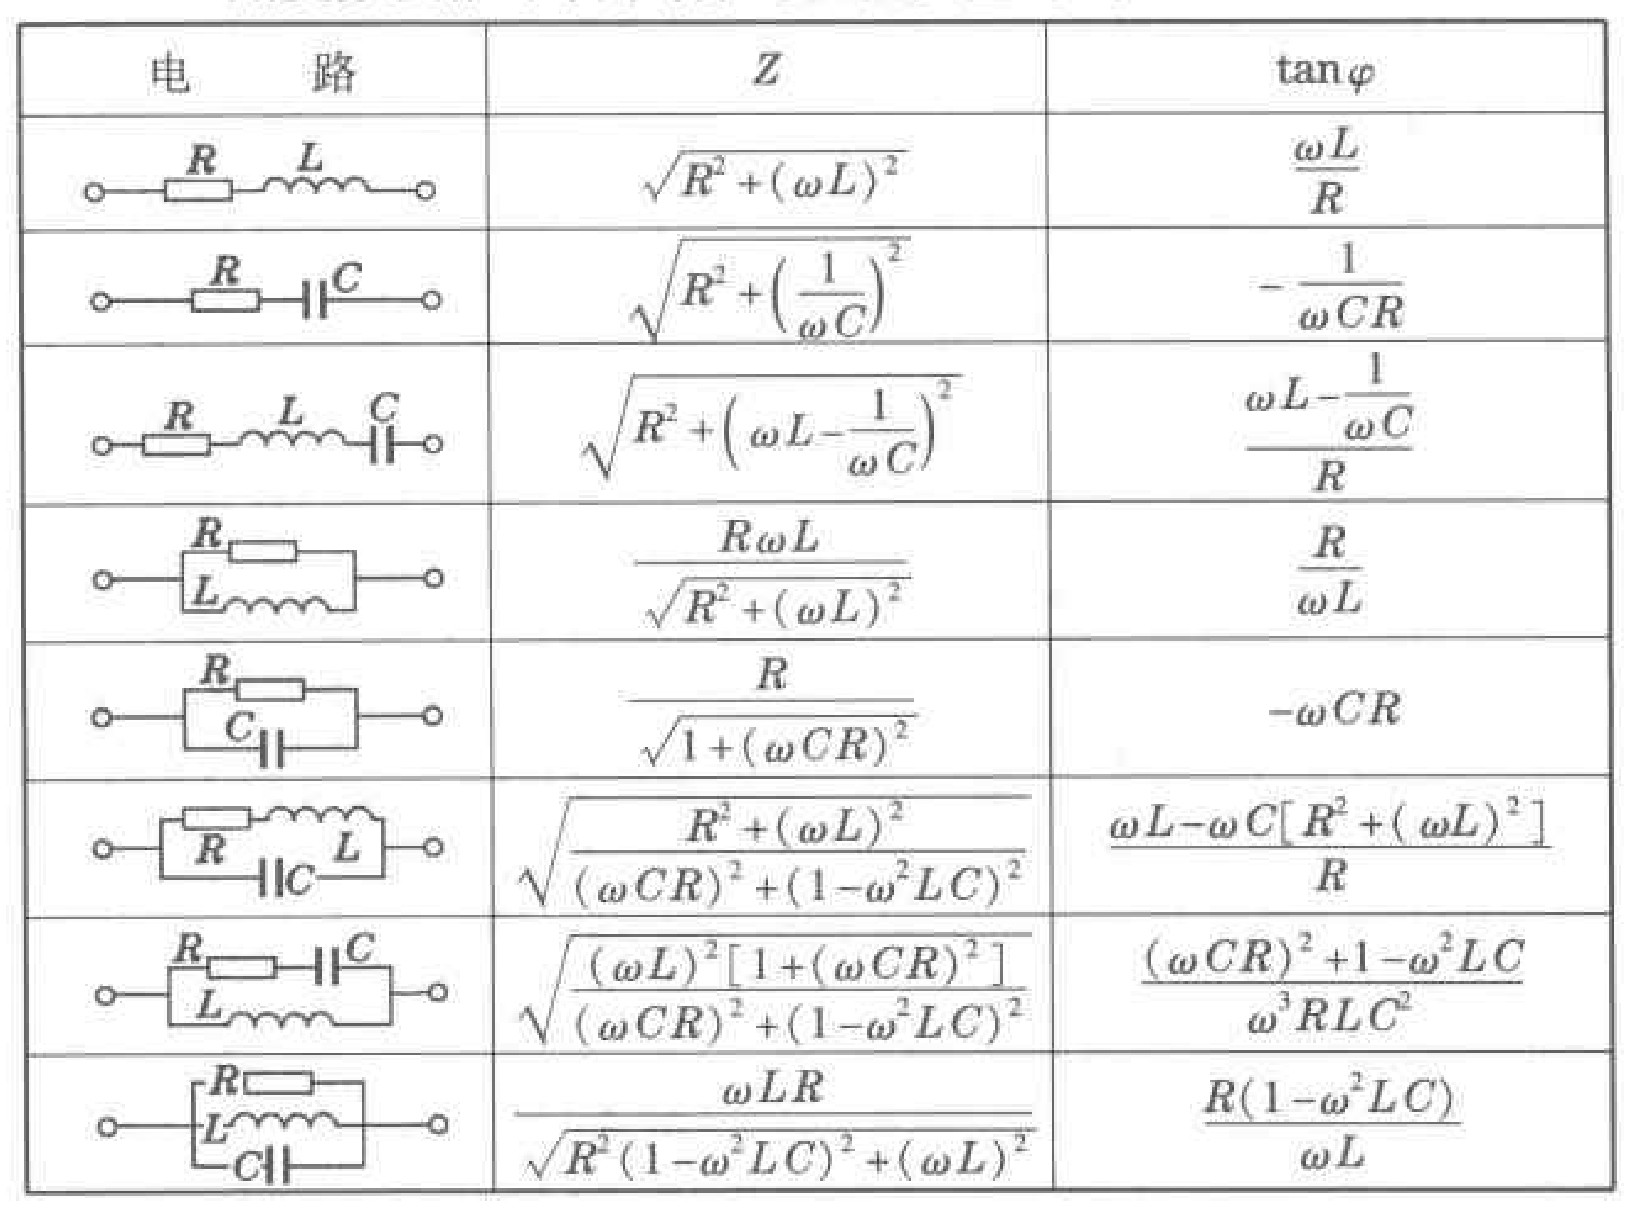
\includegraphics[width=0.6\linewidth]{figures/习题5-44.jpg}
\end{center}
\vfill
\newpage

\textbf{5-45.} 本题图中 $a$ 、 $b$ 两点接到一个交流电源上，二点间的电压为 $130\mathrm{V}$ ， $R_{1} = 6.0\Omega$ ， $R_{2} = R_{3} = 3.0\Omega$ ， $Z_{L} = 8.0\Omega$ ， $Z_{C} = 3.0\Omega$ ，求：

(1) 电路中的电流；

(2) a、c 两点间的电压；

(3) c、d 两点间的电压。
\begin{center}
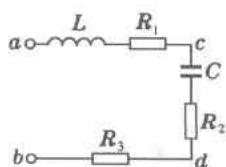
\includegraphics[width=0.25\linewidth]{figures/习题5-45.jpg}
\end{center}

\vfill
\textbf{5-46.} 一直流电阻为 $120\Omega$ 的抗流圈与一电容为 $10\mu \mathrm{F}$ 的电容器串联。当电源频率为 $50\mathrm{Hz}$ 、总电压为 $120\mathrm{V}$ 、电流为 $1.0\mathrm{A}$ 时，求抗流圈的自感。

\vfill
\newpage

\textbf{5-47.} (1)一个电阻与一个电感串联在 $100\mathrm{V}$ 的交流电源上,一个交流伏特计不论接在电阻或电感上时,读数都相等。这个读数应为多少?

(2) 改变(1)中电阻及电感的大小,使接于电感上的伏特计读数为 50V.这时若把伏特计接于电阻上,其读数是多少?

\vfill
\textbf{5-48.} 如本题图，从 $AO$ 输入的信号中，有直流电压6V，交流成分400 kHz, 现在要信号到达 BO 两端没有直流压降, 而交流成分要有 90% 以上, 为此在 AB 路上安置一个电容 C, 电容 C 在这里起什么作用? 它的容量至少该取多大?
\begin{center}
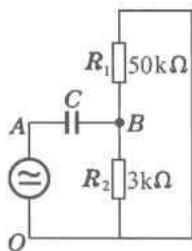
\includegraphics[width=0.25\linewidth]{figures/习题5-48.jpg}
\end{center}

\vfill
\newpage

\textbf{5-49.} 如本题图, 输入信号中包含直流成分 6V, 交流成分 500Hz、1V. 要求在 AB 两端获得直流电压 1V, 而交流电压小于 1mV, 问电阻 $R_{2}$ 该取多大, 旁路电容 C 至少该取多大?
\begin{center}
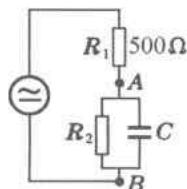
\includegraphics[width=0.25\linewidth]{figures/习题5-49.jpg}
\end{center}

\vfill
\textbf{5-50.} 本题图为测量线圈的电感量及其损耗电阻而采用的一种电桥电路。 $R_{\mathrm{s}}$ 和 $C_\mathrm{s}$ 为已知的固定电阻和电容，调节 $R_{1}, R_{2}$ 使电桥达到平衡，

(1) 求 $L_{x}$ 、 $r_{x}$ .

(2) 试比较这个电桥和图5-88所示的麦克斯韦LC电桥,哪个计算起来比较方便? 如果待测电感的等效电路采用并联式的,情况怎样?

【提示：并联式等效电路与串联式等效电路中的损耗电阻含义不同。】
\begin{center}
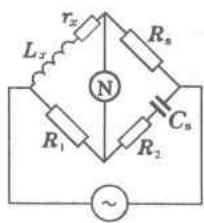
\includegraphics[width=0.25\linewidth]{figures/习题5-50.jpg}
\end{center}

\vfill
\newpage

\textbf{5-51.} 本题图是为消除分布电容的影响而设计的一种脉冲分压器。当 $C_1$ 、 $C_2$ 、 $R_{1}$ 、 $R_{2}$ 满足一定条件时，这分压器就能和直流电路一样，使输入电压 $U_{1}$ 与输出电压 $U_{2}$ 之比等于电阻之比：

$$
\frac {U _ {1}}{U _ {2}} = \frac {R _ {2}}{R _ {1} + R _ {2}},
$$

而和频率无关。试求电容、电阻应满足的条件。

\begin{center}
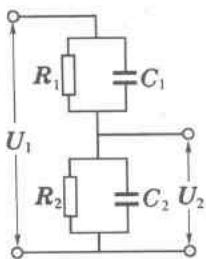
\includegraphics[width=0.25\linewidth]{figures/习题5-51.jpg}
\end{center}

\vfill
\textbf{5-52.} 在环形铁芯上绕有两个线圈，一个匝数为 $N$ ，接在电动势为 $\mathcal{E}$ 的交流电源上；另一个是均匀圆环，电阻为 $R$ ，自感很小，可略去不计。在这环上有等距离的三点： $a$ 、 $b$ 和 $c$ 。G 是内阻为 $r$ 的交流电流计。

(1) 如附图 a 连接, 求通过 G 的电流;

(2) 如附图 b 连接, 求通过 G 的电流。
\begin{center}
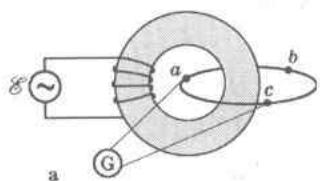
\includegraphics[width=0.25\linewidth]{figures/习题5-52a.jpg}
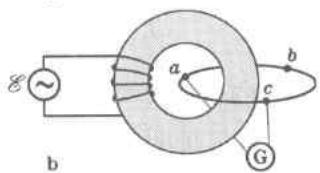
\includegraphics[width=0.25\linewidth]{figures/习题5-52b.jpg}\\
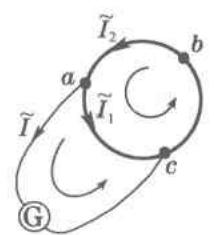
\includegraphics[width=0.25\linewidth]{figures/习题5-52c.jpg}
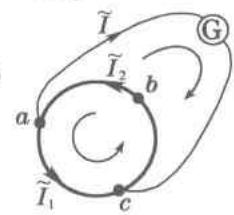
\includegraphics[width=0.25\linewidth]{figures/习题5-52d.jpg}
\end{center}

\vfill
\newpage

\textbf{5-53.} 在本题图的滤波电路中，在 $\nu = 100\mathrm{Hz}$ 的频率下欲使输出电压 $U_{2}$ 为输入电压 $U_{1}$ 的 $1 / 10$ ，求此时抗流圈自感 $L$ ，已知 $C_1 = C_2 = 10\mu \mathrm{F}$
\begin{center}
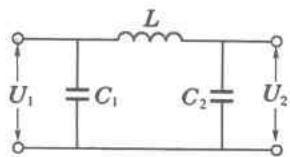
\includegraphics[width=0.3\linewidth]{figures/习题5-53.jpg}
\end{center}

\vfill
\textbf{5-54.} 本题图为电流高通型三级 $RC$ 相移电路。设输入信号电流为 $i(t) = I\cos \omega t$ ，输出信号电流为

$$
i _ {3} (t) = I \cos (\omega t + \varphi_ {3}),
$$

$\varphi_{3}$ 值为电流相移量,电流传输系数 $\eta=I_{3}/I$ .

(1) 相移量 $\varphi_{3}$ 应该是正值还是负值?

(2) 证明

$$
\widetilde {I _ {3}} = \frac {(\omega C R) ^ {3}}{\omega C R [ (\omega C R) ^ {2} - 5 ] + \mathrm{i} [ 1 - 6 (\omega C R) ^ {2} ]} \widetilde {I};
$$

(3) 算出当 $\omega CR = 1$ 时的相移量 $\varphi_{3}$ 值及传输系数 $\eta$ ;

(4) 证明：相移量达到 $\pi$ 值的频率条件为

此时 $\eta = 1/29.$

$$
\nu_ {0} = \frac {1}{2 \pi \sqrt {6} R C},
$$

(5) 已知 $R = 10 \, k\Omega, C = 0.01 \, \mu F$ ，算出振荡频率 $\nu_{0}$ .
\begin{center}
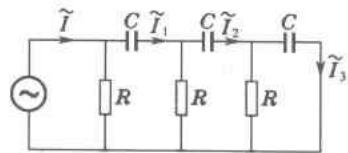
\includegraphics[width=0.3\linewidth]{figures/习题5-54.jpg}
\end{center}

\vfill
\newpage

\textbf{5-55.} 一单相电动机的铭牌告诉我们 $U = 220\mathrm{V}$ , $I = 3.0\mathrm{A}$ , $\cos \varphi = 0.8$ ，试求电动机的视在功率、有功功率和绕组的电阻。

\vfill
\textbf{5-56.} 一个 $110\mathrm{V}$ 、 $50\mathrm{Hz}$ 的交流电源供给一电路 $330\mathrm{W}$ 的功率, 功率因数 0.6, 且电流相位落后于电压。

(1) 若在电路中并联一电容器使功率因数增到 1, 求电容器的电容;

(2) 这时电源供给多少功率?

\vfill
\newpage

\textbf{5-57.} 一电路感抗 $X_{L} = 8.0\Omega$ ，电阻 $R = 6.0\Omega$ ，串接在 $220\mathrm{V}$ 、 $50\mathrm{Hz}$ 的市电上，问：

(1) 要使功率因数提高到95%，应在LR上并联多大的电容？

(2) 这时流过电容的电流是多少?

(3) 若串联电容, 情况如何?
\begin{center}
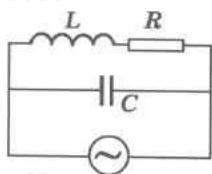
\includegraphics[width=0.25\linewidth]{figures/习题5-57a.jpg}
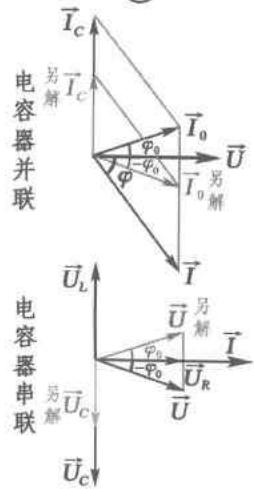
\includegraphics[width=0.17\linewidth]{figures/习题5-57b.jpg}
\end{center}

\vfill
\textbf{5-58.} 一发电机沿干线输送电能给用户，此发电机电动势为 $\mathcal{E}$ ，角频率为 $\omega$ ，干线及发电机的电阻和电感各为 $R_{0}$ 和 $L_{0}$ ，用户电路中的电阻和电感各为 R 和 L，求：

(1) 电源所供给的全部功率 P;

(2) 用户得到的功率 $P'$ ;

(3) 整个装置的效率 $\eta = P' / P$ .
\begin{center}
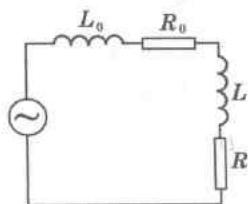
\includegraphics[width=0.3\linewidth]{figures/习题5-58.jpg}
\end{center}

\vfill
\newpage

\textbf{5-59.} 输电干线的电压 $U = 120\mathrm{V}$ ，频率为 $50.0\mathrm{Hz}$ 。用户照明电路与抗流圈串联后接于干线间，抗流圈的自感 $L = 0.0500\mathrm{H}$ ，电阻 $R = 1.00\Omega$ （见本题图），问：

(1) 当用户共用电 $I_{0}=2.00A$ 时，他们电灯两端的电压 $U'$ 等于多少？

(2) 用户电路(包括抗流圈在内)能得到最大的功率是多少?

(3) 当用户电路中发生短路时,抗流圈中消耗功率多少?
\begin{center}
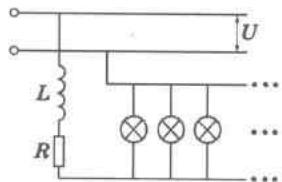
\includegraphics[width=0.3\linewidth]{figures/习题5-59.jpg}
\end{center}

\vfill
\textbf{5-60.} 本题图中已知电阻 $R = 20\Omega$ ，三个伏特计 $\mathrm{V}_{1}, \mathrm{V}_{2}, \mathrm{V}$ 的读数分别为 $U_{1} = 91\mathrm{V}, U_{2} = 44\mathrm{V}, U = 120\mathrm{V}$ ，求元件 $Z$ 中的功率。
\begin{center}
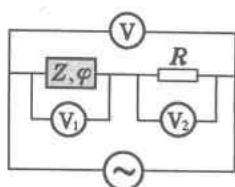
\includegraphics[width=0.25\linewidth]{figures/习题5-60a.jpg}
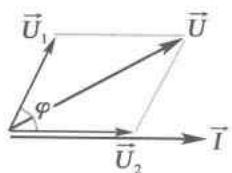
\includegraphics[width=0.25\linewidth]{figures/习题5-60b.jpg}
\end{center}

\vfill
\newpage

\textbf{5-61.} 本题图中已知电阻 $R = 50\Omega$ ，三个电流计 $\mathrm{A}_1$ 、 $\mathrm{A}_2$ 、A的读数分别为 $I_{1} = 2.8\mathrm{A}$ ， $I_{2} = 2.5\mathrm{A}$ ， $I = 4.5\mathrm{A}$ ，求元件 $Z$ 中的功率。
\begin{center}
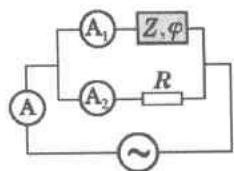
\includegraphics[width=0.25\linewidth]{figures/习题5-61a.jpg}
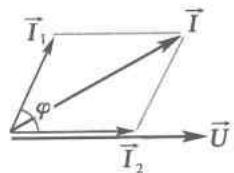
\includegraphics[width=0.25\linewidth]{figures/习题5-61b.jpg}
\end{center}

\vfill
\textbf{5-62.} 一个 $RLC$ 串联电路如本题图，已知 $R = 300\Omega, L = 250\mathrm{mH}$ ， $C = 8.00\mu \mathrm{F}$ ，A 是交流安培计， $\mathrm{V}_{1}, \mathrm{V}_{2}, \mathrm{V}_{3}, \mathrm{V}_{4}$ 和 V 都是交流伏特计。现在把 $a, b$ 两端分别接到市电（220V、50Hz）电源的两极上。

(1) 问 A、 $V_{1}$ 、 $V_{2}$ 、 $V_{3}$ 、 $V_{4}$ 和 V 的读数各多少?

(2) 求 a、b 间消耗的功率。
\begin{center}
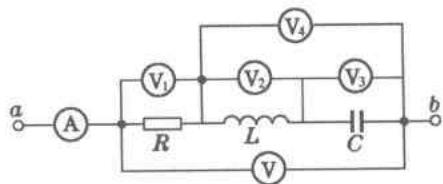
\includegraphics[width=0.4\linewidth]{figures/习题5-62.jpg}
\end{center}

\vfill
\newpage

\textbf{5-63.} 计算 $LR$ 并联电路的有功电阻 $r$ .

\vfill
\textbf{5-64.} 平行板电容器中的电介质介电常量 $\varepsilon = 2.8$ ，因电介质漏电而使电容器在 $50\mathrm{Hz}$ 的频率下有损耗角 $\delta = 1^{\circ}$ ，求电介质的电阻率。

\vfill
\newpage

\textbf{5-65.} 在一电感线圈的相邻匝与匝间，不相邻匝与匝间，接线端间，与地间都存在小的“分布电容”。这许多小电容的总效应可以用一个适当大小$C _ {0}$电容的数值取决于线圈的尺寸及绕法。分布电容的效应在频率愈高时愈显著（根据图a分析一下，为什么？），试证明：如果我们仍把电感线圈看成纯电感 $L'$ 和有功电阻 $r'$ 串联的话（见图b），由于存在分布电容 $C_0$ ，则

$$
L ^ {\prime}  = \frac {L}{1 - \omega^ {2} L C _ {0}}, r ^ {\prime} = \frac {r}{(1 - \omega^ {2} L C _ {0}) ^ {2}}
$$

从而$Q ^ {\prime}  = \frac {\omega L ^ {\prime}}{r ^ {\prime}} = Q (1 - \omega^ {2} L C _ {0}).$

即线圈的表观电感 $L'$ 增加，而表观Q值下降（设 $Q\gg1$ ）。
\begin{center}
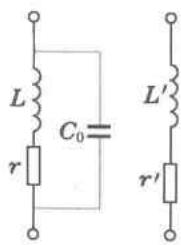
\includegraphics[width=0.2\linewidth]{figures/习题5-65.jpg}
\end{center}

\vfill
\textbf{5-66.} 串联谐振电路中 $L = 0.10\mathrm{H}$ , $C = 25.0\mathrm{pF}$ , $R = 10\Omega$

(1) 求谐振频率；

(2) 若总电压为 $50 \, mV$ ，求谐振时电感元件上的电压。

\vfill
\newpage

\textbf{5-67.} 串联谐振电路接在 $\mathcal{E} = 5.0\mathrm{V}$ 的电源上，谐振时电容器上的电压等于 $150\mathrm{V}$ ，求 $Q$ 值。

\vfill
\textbf{5-68.} 串联谐振电路的谐振频率 $\nu_{0} = 600\mathrm{kHz}$ , 电容 $C = 370\mathrm{pF}$ , 这频率下电路的有功电阻 $r = 15\Omega$ , 求电路的 $Q$ 值。

\vfill
\newpage

\textbf{5-69.} 将一个输入 $220 \mathrm{~V}$ 、输出 $6.3 \mathrm{~V}$ 的变压器改绕成输入 $220 \mathrm{~V}$ 、输出 $30 \mathrm{~V}$ 的变压器，现拆出次级线圈，数出圈数是38匝，应改绕成多少匝？

\vfill
\textbf{5-70.} 有一变压器能将 $100\mathrm{V}$ 升高到 $3300\mathrm{V}$ . 将一导线绕过其铁芯, 两端接在伏特计上 (见本题图)。此伏特计的读数为 $0.5\mathrm{V}$ , 问变压器二绕组的匝数 (设变压器是理想的)。
\begin{center}
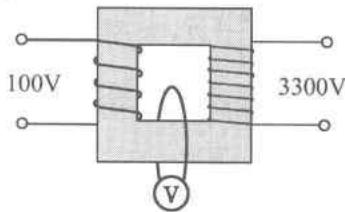
\includegraphics[width=0.4\linewidth]{figures/习题5-70.jpg}
\end{center}

\vfill
\newpage

\textbf{5-71.} 理想变压器匝数比 $N_{2} / N_{1} = 10$ ，交流电源电压为 $110\mathrm{V}$ ，负载 $1.0\mathrm{k}\Omega$ ，求两线圈中的电流。

\vfill
\textbf{5-72.} 某电源变压器的原线圈是660匝，接在电压为 $220\mathrm{V}$ 的电源上，问：

（1）要在三个副线圈上分别得到5.0V、6.3V和350V的电压，三个副线圈各应绕多少匝？

（2）设通过三个副线圈的电流分别是3.0A、3.0A和280mA，通过原线圈的电流是多少？

\vfill
\newpage

\textbf{5-73.} 如本题图所示, 输出变压器的次级有中间抽头, 以便接 $3.5 \Omega$ 的扬声器或接 $8 \Omega$ 的扬声器都能使阻抗匹配, 次级线圈两部分匝数之比 $N_{1} / N_{2}$ 应为多少?
\begin{center}
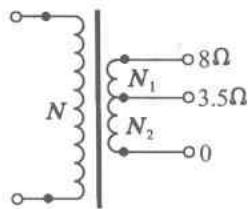
\includegraphics[width=0.2\linewidth]{figures/习题5-73.jpg}
\end{center}

\vfill
\textbf{5-74.} 若需绕制一个电源变压器，接 $220\mathrm{V}$ 、 $50\mathrm{Hz}$ 的输入电压，要求有 $40\mathrm{V}$ 和 $6\mathrm{V}$ 的两组输出电压，试问原线圈及两组副线圈的匝数。已知铁芯的截面积为 $8.0\mathrm{cm}^2$ ，最大磁感应强度 $B_{\mathrm{max}}$ 选取12000Gs.

\vfill
\newpage

\textbf{5-75.} 在可控硅的控制系统中常用到 $RC$ 移相电桥电路（见本题图），电桥的输入电压由变压器次级提供，输出电压从变压器中心抽头 $O$ 和 $D$ 之间得到。试证明输出电压 $\widetilde{U}_{OD}$ 的相位随 $R$ 改变，但其大小保持不变。
\begin{center}
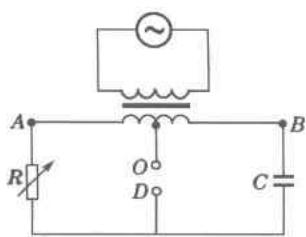
\includegraphics[width=0.3\linewidth]{figures/习题5-75a.jpg}
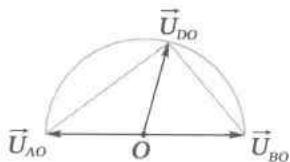
\includegraphics[width=0.3\linewidth]{figures/习题5-75b.jpg}
\end{center}

\vfill
\textbf{5-76.} 导纳电桥的原理性电路如本题图所示, 其中两个臂1和2是有抽头的变压器副线圈, 电源通过这变压器耦合起来。另外两个臂一个是电阻 $R$ , 一个是电容 $C$ 和待测电感元件(其等效电路示于右旁阴影区内)的并联,R 和 C 都是可调的。试证明：电桥达到平衡时，待测电感元件的 Q 值可通过下式算出：

$$
Q = \frac {N _ {1}}{N _ {2}} \frac {1}{\omega C R},
$$

其中 $N_{1}, N_{2}$ 分别是 1、2 两臂的匝数。

若等效电路设为 $R_{x}$ 与 $L_{x}$ 串联，Q的表达式如何？
\begin{center}
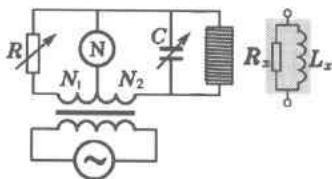
\includegraphics[width=0.4\linewidth]{figures/习题5-76.jpg}
\end{center}

\vfill
\newpage

\textbf{5-77.} 有一星形连接的三相对称负载(电动机), 每相的电阻为 $R = 6.0 \Omega$ , 电抗为 $X = 8.0 \Omega$ ; 电源的线电压为 $380 \mathrm{~V}$ , 求:

(1) 线电流；

(2) 负载所消耗的功率；

(3) 如果改接成三角形, 求线电流和负载所消耗的功率。

\vfill
\textbf{5-78.} 三相交流电的线电压为 $380\mathrm{V}$ ，负载是不对称的纯电阻， $R_{A} = R_{B} = 22\Omega$ ， $R_{C} = 27.5\Omega$ ，作星形连接。

(1) 求中线电流；

(2) 求各相的相电压；

(3) 若中线断开, 各相电压将变为多少?
\begin{center}
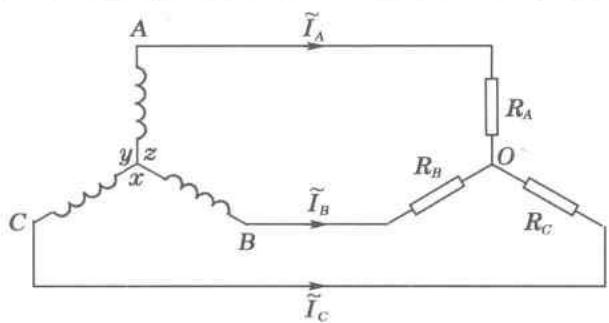
\includegraphics[width=0.35\linewidth]{figures/习题5-78a.jpg}
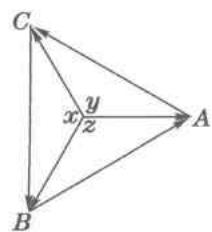
\includegraphics[width=0.18\linewidth]{figures/习题5-78b.jpg}
\end{center}

\vfill
\newpage